\documentclass[11pt,a4paper]{article}
\usepackage[T1]{fontenc}
\usepackage[utf8]{inputenc}
\usepackage[spanish,es-nodecimaldot,es-noshorthands]{babel}
\usepackage[default]{sourcesanspro}
\usepackage{amsmath,amssymb,graphicx,booktabs,tabularx,array,parskip,enumitem}
\usepackage{microtype,xcolor,tcolorbox,fancyhdr,lastpage,caption}
\usepackage[margin=19mm,headheight=16pt,headsep=7mm,footskip=10mm]{geometry}
\definecolor{navy}{HTML}{18354A}
\definecolor{teal}{HTML}{087F8C}
\definecolor{ink}{HTML}{253746}
\definecolor{muted}{HTML}{536675}
\definecolor{pale}{HTML}{EFF6F8}
\usepackage[colorlinks=true,linkcolor=teal,urlcolor=teal,bookmarksopen=true]{hyperref}
\hypersetup{pdftitle={Siete maestros de coloración con E1: resultados y adaptaciones},
  pdfsubject={Seguimiento experimental e1-native-v1, 22 de octubre de 2026},pdfauthor={}}
\urlstyle{same}
\pagestyle{fancy}
\fancyhf{}
\fancyhead[L]{\small\color{muted}SIETE MAESTROS DE COLORACIÓN}
\fancyhead[R]{\small\color{teal}E1 / ADAPTADA}
\fancyfoot[L]{\footnotesize\color{muted}22 de octubre de 2026 · e1-native-v1}
\fancyfoot[R]{\footnotesize\color{muted}\thepage\ / \pageref*{LastPage}}
\renewcommand{\headrulewidth}{0.3pt}
\renewcommand{\footrulewidth}{0pt}
\setlength{\parindent}{0pt}
\setlength{\parskip}{5pt}
\setlength{\emergencystretch}{2em}
\setlength{\tabcolsep}{5pt}
\renewcommand{\arraystretch}{1.17}
\setlist[itemize]{leftmargin=*,topsep=3pt,itemsep=3pt,parsep=0pt}
\captionsetup{font=small,labelfont=bf,justification=raggedright,singlelinecheck=false,skip=4pt,hypcap=false}
\newcolumntype{Y}{>{\raggedright\arraybackslash}X}
\newcommand{\pageheading}[2]{\pdfbookmark[0]{#2}{page#1}%
  {\small\bfseries\color{teal}#1\par}\vspace{2mm}%
  {\fontsize{22}{25}\selectfont\bfseries\color{navy}#2\par}\vspace{3mm}}
\newcommand{\subhead}[1]{\vspace{2mm}{\large\bfseries\color{navy}#1\par}\vspace{1mm}}
\newtcolorbox{finding}{colback=pale,colframe=teal,boxrule=0pt,leftrule=2pt,
  arc=0pt,left=3mm,right=3mm,top=2mm,bottom=2mm,before skip=5pt,after skip=6pt}
\newcommand{\file}[1]{{\small\nolinkurl{#1}}}
% Generated from the frozen CSVs; do not edit manually.
\newcommand{\LearnedRuns}{13\,860}
\newcommand{\LearnedSuccesses}{13\,482}
\newcommand{\TotalSuccessPercent}{97{,}27}
\newcommand{\LearnedFailures}{378}
\newcommand{\ResultRows}{
Luby & 1\,857 & 1\,980 & 100{,}00 & +6{,}21 \\
Johansson & 1\,919 & 1\,980 & 100{,}00 & +3{,}08 \\
Jones--Plassmann & 1\,635 & 1\,631 & 82{,}37 & -0{,}20 \\
ColorTrials repetido & 1\,980 & 1\,980 & 100{,}00 & +0{,}00 \\
BE (base $\Delta\leq3$) & 872 & 1\,980 & 100{,}00 & +55{,}96 \\
Especulativo GM & 1\,975 & 1\,951 & 98{,}54 & -1{,}21 \\
Greedy secuencial & 1\,842 & 1\,980 & 100{,}00 & +6{,}97 \\
}
\newcommand{\LargeSizeRows}{
Luby & 23 & 30 & 6 & 30 \\
Johansson & 28 & 30 & 16 & 30 \\
Jones--Plassmann & 10 & 0 & 8 & 2 \\
ColorTrials repetido & 30 & 30 & 30 & 30 \\
BE (base $\Delta\leq3$) & 0 & 30 & 0 & 30 \\
Especulativo GM & 30 & 30 & 30 & 25 \\
Greedy secuencial & 30 & 30 & 18 & 30 \\
}
\newcommand{\MilestoneRows}{
Luby & 17\,760 & 100 & 99{,}8437 \\
Johansson & No alcanzado & 100 & 99{,}8173 \\
Jones--Plassmann & No alcanzado & No alcanzado & 99{,}9735 \\
ColorTrials repetido & 500 & 500 & 100{,}0000 \\
BE (base $\Delta\leq3$) & No alcanzado & 4\,000 & 100{,}0000 \\
Especulativo GM & 8\,000 & 500 & 100{,}0000 \\
Greedy secuencial & No alcanzado & 100 & 100{,}0000 \\
}


\begin{document}
\color{ink}

\pageheading{01 · RESULTADO PRINCIPAL}{Cómo aprende la GNN con siete maestros}

Entrenamos desde cero \textbf{35 redes: siete maestros y cinco inicializaciones}
por maestro. Cada red aprende con grafos de 40 nodos y se prueba hasta
10.240 nodos, con grado máximo a lo sumo 3 y una paleta común de cuatro colores.
La referencia anterior usaba otra GNN, de 36.719 parámetros.

\begin{finding}
\textbf{Luby, Johansson, ColorTrials, BE y greedy completan todos sus casos.}
En conjunto, E1 y sus adaptaciones logran \LearnedSuccesses/\LearnedRuns{}
coloraciones correctas (\TotalSuccessPercent\,\%). JP y GM concentran los
\LearnedFailures{} fallos: todos quedan incompletos, sin colisiones observadas.
\end{finding}

{\small\textbf{Éxitos de 1.980 ejecuciones por maestro.}
Cada cifra agrega cinco inicializaciones sobre los mismos 396 casos.}
\begin{center}\small
\begin{tabularx}{\linewidth}{@{}Yrrrr@{}}
\toprule
Maestro & GNN anterior & E1 / adaptada & Éxito (\%) & Cambio (pp)\\
\midrule
\ResultRows
\bottomrule
\end{tabularx}
\end{center}

\begin{center}
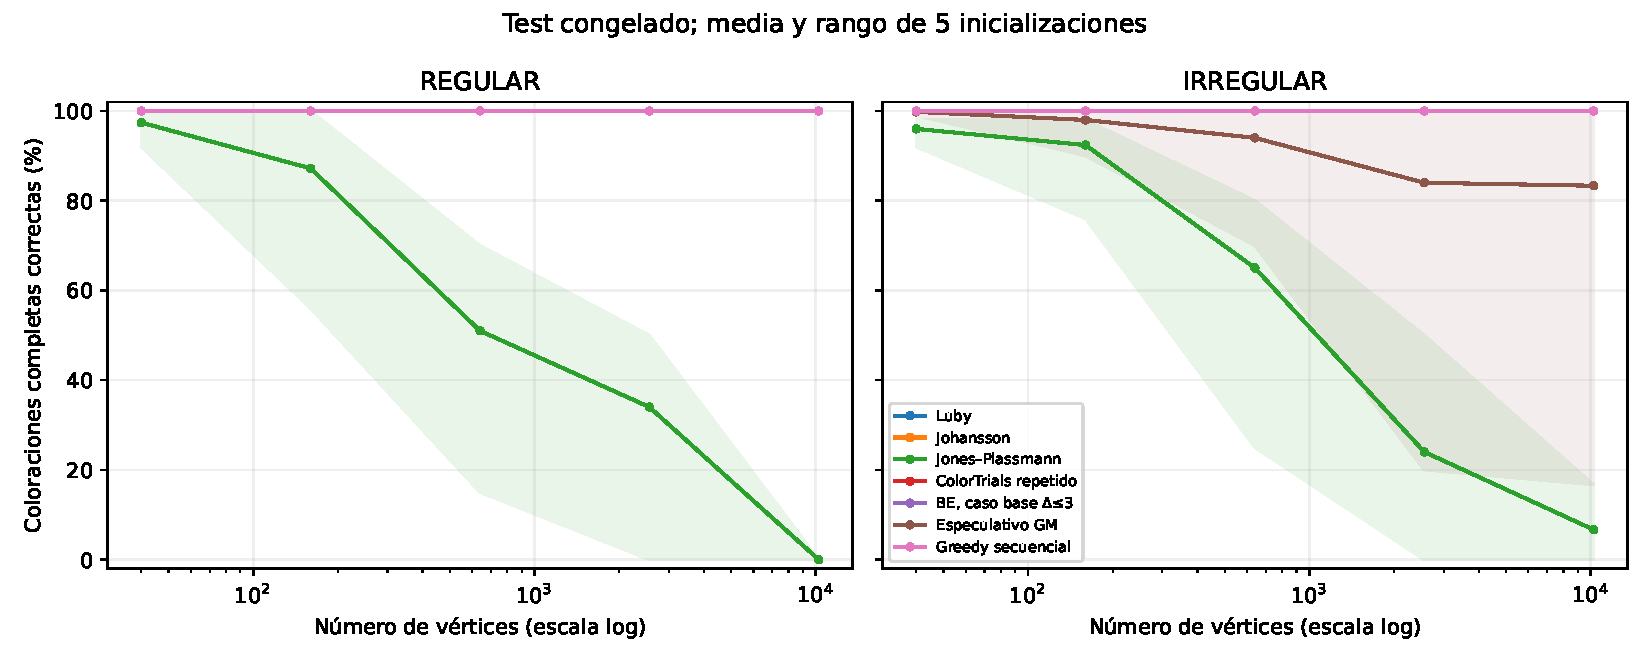
\includegraphics[width=\linewidth]{success-by-size.pdf}
\captionof{figure}{Éxito autónomo según tamaño en la nueva cohorte. Las bandas
son el rango entre inicializaciones, no intervalos de confianza. Varias curvas
coinciden en el 100\,\%.}
\end{center}

\textbf{Qué significa «E1 modificada».} Luby, Johansson y greedy usan el núcleo
original de 16.035 parámetros. JP, ColorTrials, BE y GM añaden adaptadores y
suman 19.396. También cambia el protocolo de entrenamiento respecto de E1
canónica. La página 2 detalla estas diferencias.

{\small\color{muted}Seguimiento exploratorio sobre casos de test ya publicados.
La comparación mide arquitectura, representación y entrenamiento en conjunto;
no estima el efecto causal de cambiar solo la arquitectura.}

\clearpage
\pageheading{02 · QUÉ ES E1 / ADAPTADA}{El núcleo se conserva; el experimento cambia}

\textbf{E1 canónica} nombra un experimento: \texttt{UniversalColorGNN}, variante
\texttt{NORMALIZED}, entrenada con supervisión contrafactual de Luby.
No basta conservar su clase para repetir exactamente ese experimento.

Aquí se conserva el núcleo de \textbf{16.035 parámetros}: pesos compartidos
entre nodos y colores, estado por nodo/color, dos intercambios de mensajes,
agregación MAX, disponibilidad aprendida y prefijos normalizados. Sus fuentes
originales permanecen intactos. Cada réplica aprende pesos nuevos.

\subhead{Cambios específicos para cada maestro}
\begingroup\small
\begin{tabularx}{\linewidth}{@{}p{27mm}rY@{}}
\toprule
Maestro & Parámetros & Información y decisiones de esta implementación\\
\midrule
Luby & 16.035 & Entradas originales; aprende participación, candidato y confirmación.\\
Johansson & 16.035 & Mismo núcleo; se enseña participación constante en nodos habilitados.\\
Greedy & 16.035 & Un calendario externo elige el único nodo habilitado; la red aprende su decisión local.\\
Jones--Plassmann & 19.396 & Diferencias de identificadores; participación después del primer mensaje para aprender la prioridad local.\\
ColorTrials & 19.396 & Preferencias por color y disponibilidad aprendida; el candidato se elige después del segundo intercambio.\\
BE, base $\Delta\leq3$ & 19.396 & Fases Linial/KW y comparaciones auxiliares. Aprende el punto $x$; el adaptador calcula $p_v(x)$. En KW aprende participación, opción y confirmación.\\
Especulativo GM & 19.396 & Fases de asignación, detección y reparación; comparación de posición en el calendario e identificadores. Aprende la marca de conflicto.\\
\bottomrule
\end{tabularx}
\endgroup

Los cuatro modelos extendidos agregan \textbf{3.361 parámetros}: módulos de
contexto en los dos mensajes, dos aportes al estado y una cabeza adicional de
participación. Comparten la misma arquitectura de adaptadores y la misma
inicialización entre maestros para cada semilla; después se entrenan por separado.
Las entradas que un maestro no usa se anulan.

\begin{finding}
\textbf{La adaptación de BE cambia sustancialmente lo aprendido.} La red
anterior elegía entre 169 pares. Ahora elige $x$ y recibe calculado el par
$(x,p_v(x))$. Es una restricción y una ayuda de representación adicionales;
la subida de 872 a 1.980 éxitos no puede atribuirse solo al núcleo E1.
\end{finding}

\subhead{Diferencias con el entrenamiento E1 original}
El original usa 120 épocas, lotes de 128 rondas y contrafactuales sobre grafos
completos. Este seguimiento conserva el presupuesto de la comparación anterior:
17.760 actualizaciones de 1.680 decisiones locales, con contrafactuales por
estrella. También conserva su intérprete nativo, sus fases y sus calendarios.
En ColorTrials, además, el gradiente de confirmación alcanza la disponibilidad
aprendida transmitida: cambia el flujo de cálculo.

{\small\color{muted}Nombre preciso: «núcleo E1 con adaptaciones nativas,
protocolo e1-native-v1». Las cuatro extensiones no son checkpoints E1 canónicos;
las otras tres tampoco reproducen por sí solas el entrenamiento original.}

\clearpage
\pageheading{03 · TRANSFERENCIA EN TAMAÑO}{La media global oculta el problema de JP}

\begin{center}
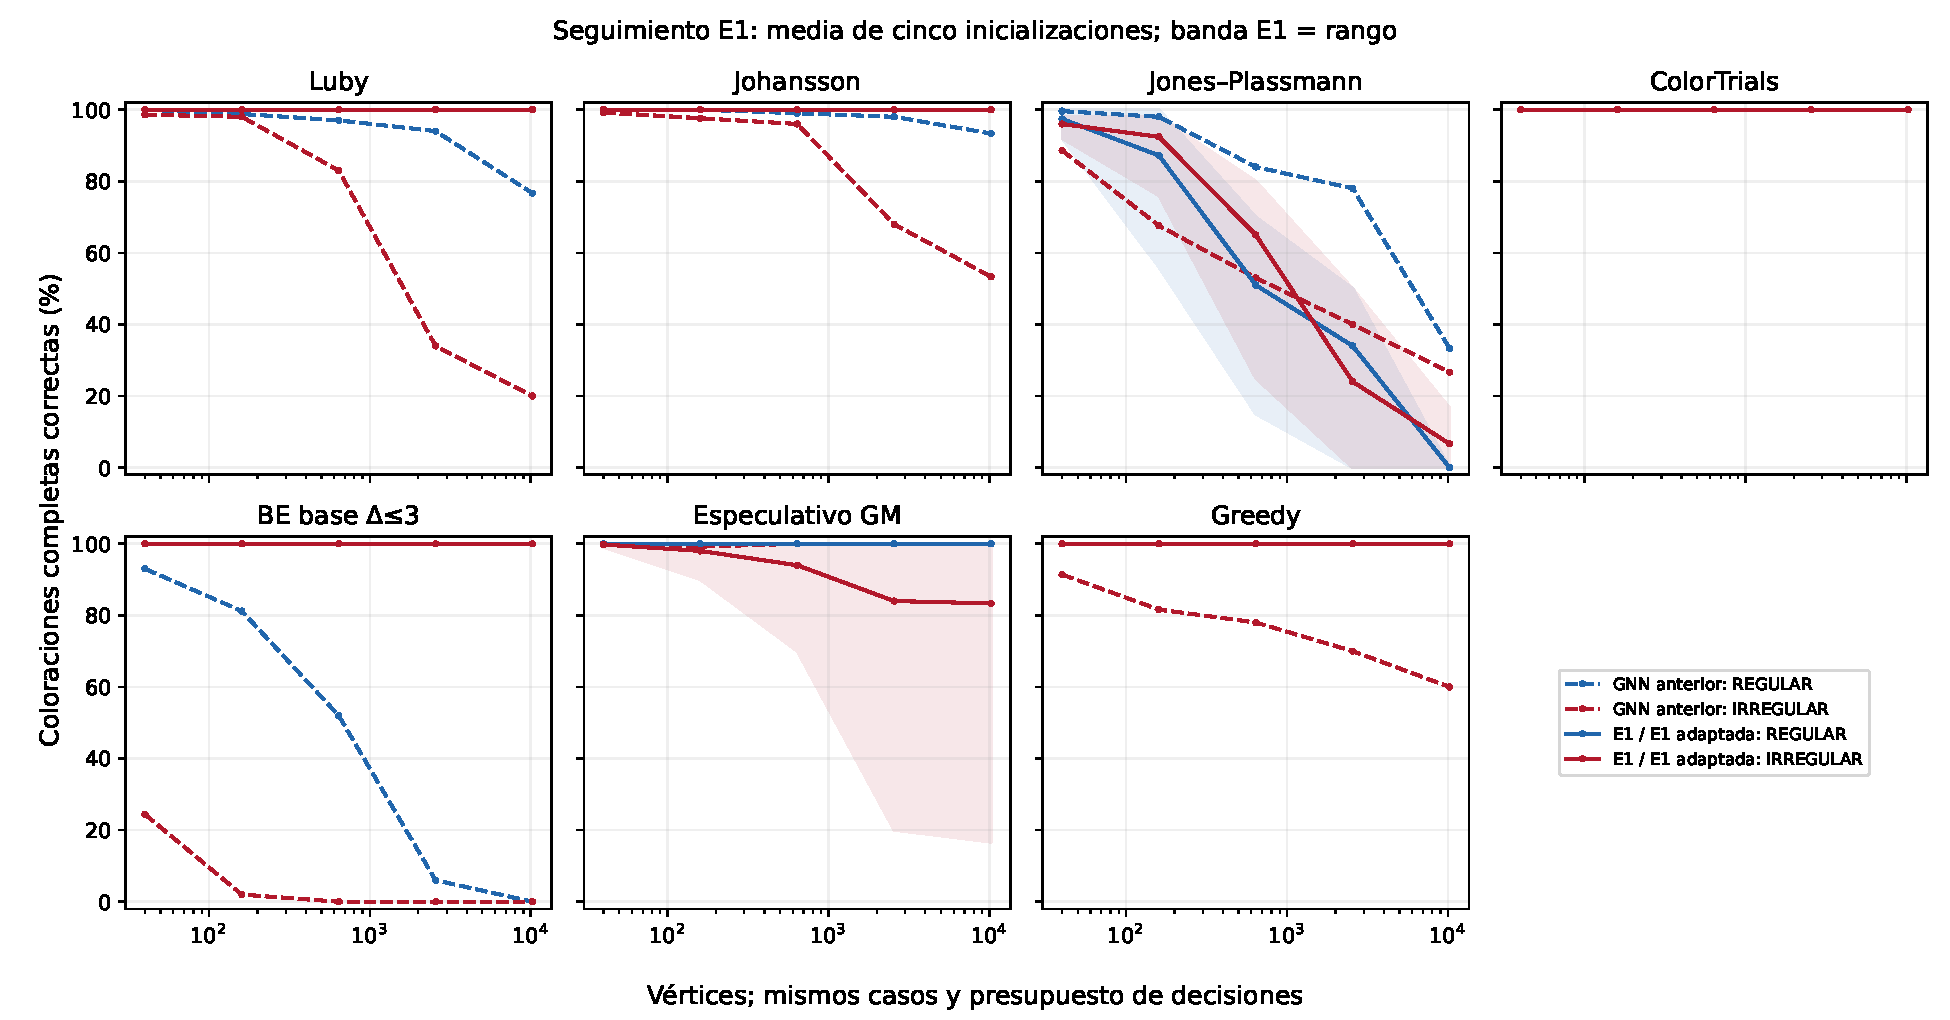
\includegraphics[width=\linewidth]{architecture-comparison.pdf}
\captionof{figure}{Antes y después, maestro por maestro. Línea discontinua:
GNN anterior; continua: E1 / adaptada. Azul: REGULAR; rojo: IRREGULAR. Las bandas
de la nueva cohorte muestran el rango entre cinco inicializaciones.}
\end{center}

\textbf{En 10.240 nodos: éxitos de 30 ejecuciones por familia.}
Son tres grafos por familia, dos tapes y cinco inicializaciones; las 30
ejecuciones comparten esos tres grafos.
\begin{center}\small
\begin{tabularx}{\linewidth}{@{}Yrrrr@{}}
\toprule
& \multicolumn{2}{c}{REGULAR} & \multicolumn{2}{c}{IRREGULAR}\\
Maestro & Anterior & E1 / adaptada & Anterior & E1 / adaptada\\
\midrule
\LargeSizeRows
\bottomrule
\end{tabularx}
\end{center}

\begin{finding}
\textbf{JP empeora al extrapolar.} Su total apenas cambia (1.635 a 1.631),
pero en 10.240 nodos pasa de 10/30 a 0/30 en REGULAR y de 8/30 a 2/30 en
IRREGULAR. Los muchos casos pequeños dominan el agregado.
\end{finding}

\textbf{GM también retrocede:} 1.951 éxitos frente a 1.975. Sus 29 fallos
nuevos quedan incompletos; JP aporta otros 349. La clasificación final del fallo
no identifica por sí sola qué decisión interna causa cada bloqueo.

{\small\color{muted}Estas curvas evalúan transferencia en número de nodos,
manteniendo la cota de grado y la paleta. No son un estudio de transferencia
a grados mayores ni una demostración de corrección universal.}

\clearpage
\pageheading{04 · CURVAS DE APRENDIZAJE}{Aprender antes no garantiza extrapolar mejor}

\begin{center}
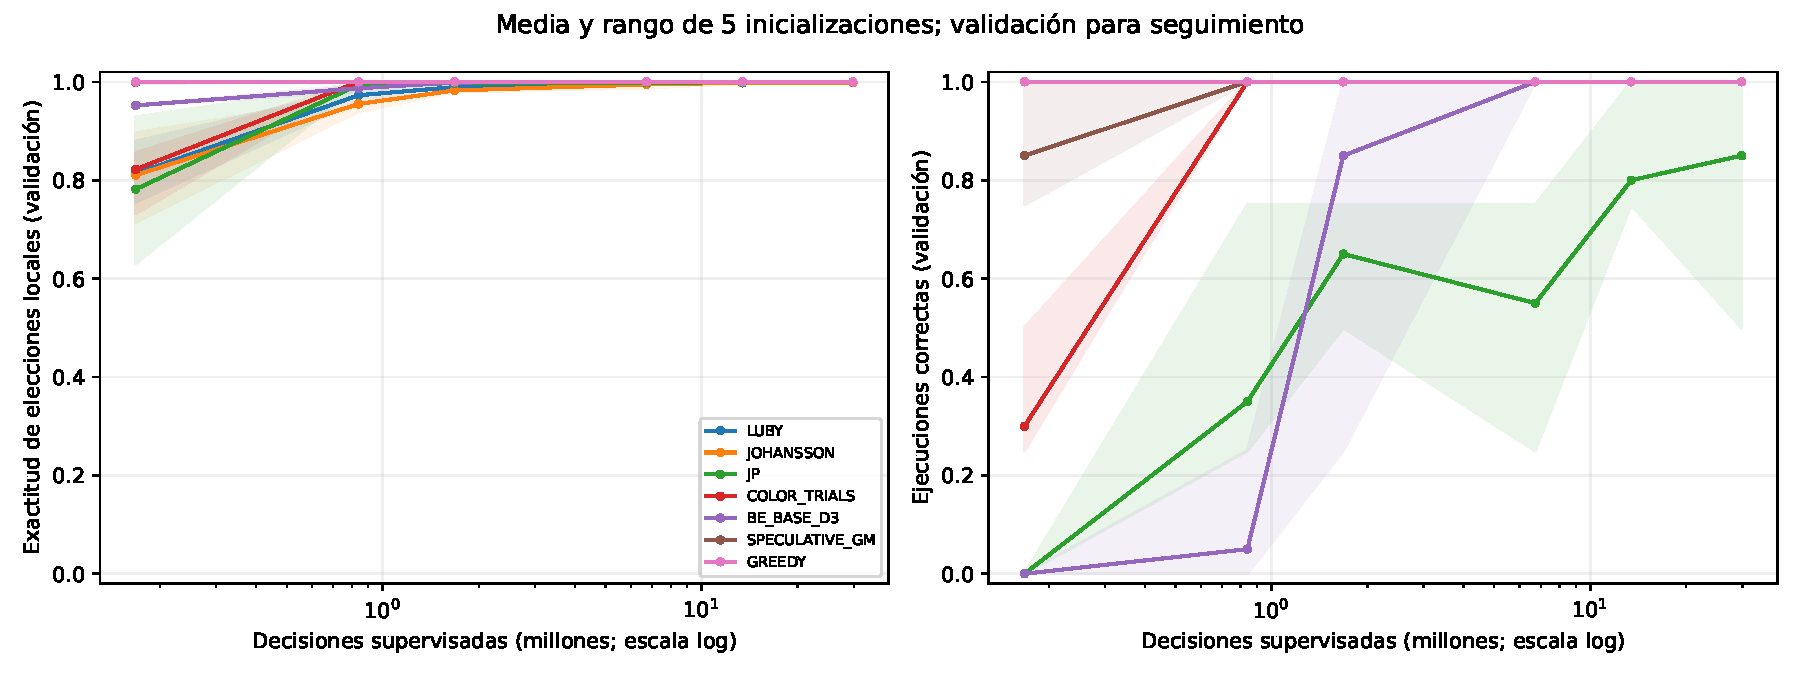
\includegraphics[width=\linewidth]{learning-curves.pdf}
\captionof{figure}{Nueva cohorte: acuerdo local con el maestro (izquierda) y
coloraciones autónomas correctas en seguimiento (derecha). Media y rango de
cinco inicializaciones; eje horizontal logarítmico, en millones de decisiones
muestreadas. Las curvas superpuestas pueden ocultarse entre sí.}
\end{center}

\subhead{Primer hito con seguimiento completo y sostenido}
La tabla indica la primera actualización observada con \textbf{20/20 éxitos}
que se conserva en todos los hitos posteriores. Esos 20 rollouts corresponden
a \textbf{cuatro grafos compartidos}, de 40/160 nodos y ambas familias, evaluados
por las cinco inicializaciones. No equivalen a 20 grafos independientes.

\begin{center}\small
\begin{tabularx}{\linewidth}{@{}Yrrr@{}}
\toprule
Maestro & Anterior & E1 / adaptada & Acuerdo local final (\%)\\
\midrule
\MilestoneRows
\bottomrule
\end{tabularx}
\end{center}

\begin{finding}
\textbf{Luby, Johansson y greedy alcanzan el seguimiento completo en el primer
hito, a 100 actualizaciones.} ColorTrials lo alcanza a 500, como antes; GM
pasa de 8.000 a 500 y BE llega a 4.000. JP no mantiene 20/20. Los siete
resultados finales se miden a 17.760, sin elegir el mejor checkpoint.
\end{finding}

\textbf{Precisión local y éxito global son medidas distintas.} JP logra
99,9735\,\% de acuerdo local final y GM 100\,\%, pero ambos fallan en ejecuciones
autónomas. La validación local consulta estados del maestro; durante el rollout,
la red visita estados producidos por sus propias decisiones, incluso errores.

Un candidato distinto del maestro puede ser un color válido. Por eso un acuerdo
local inferior al 100\,\% puede coexistir con todos los rollouts correctos,
como ocurre con Luby y Johansson. A la inversa, el acuerdo en estados observados
no certifica terminación ni cubre todos los estados propios.

{\small\color{muted}Hitos registrados: 100, 500, 1.000, 4.000, 8.000 y 17.760.
La tabla describe esos puntos discretos; no mide el instante exacto en que se
adquiere una regla ni permite convertir actualizaciones en tiempo de ejecución.}

\clearpage
\pageheading{05 · FASES Y SUPERVISIÓN}{Qué aprende la red y qué aporta el intérprete}

\begin{center}
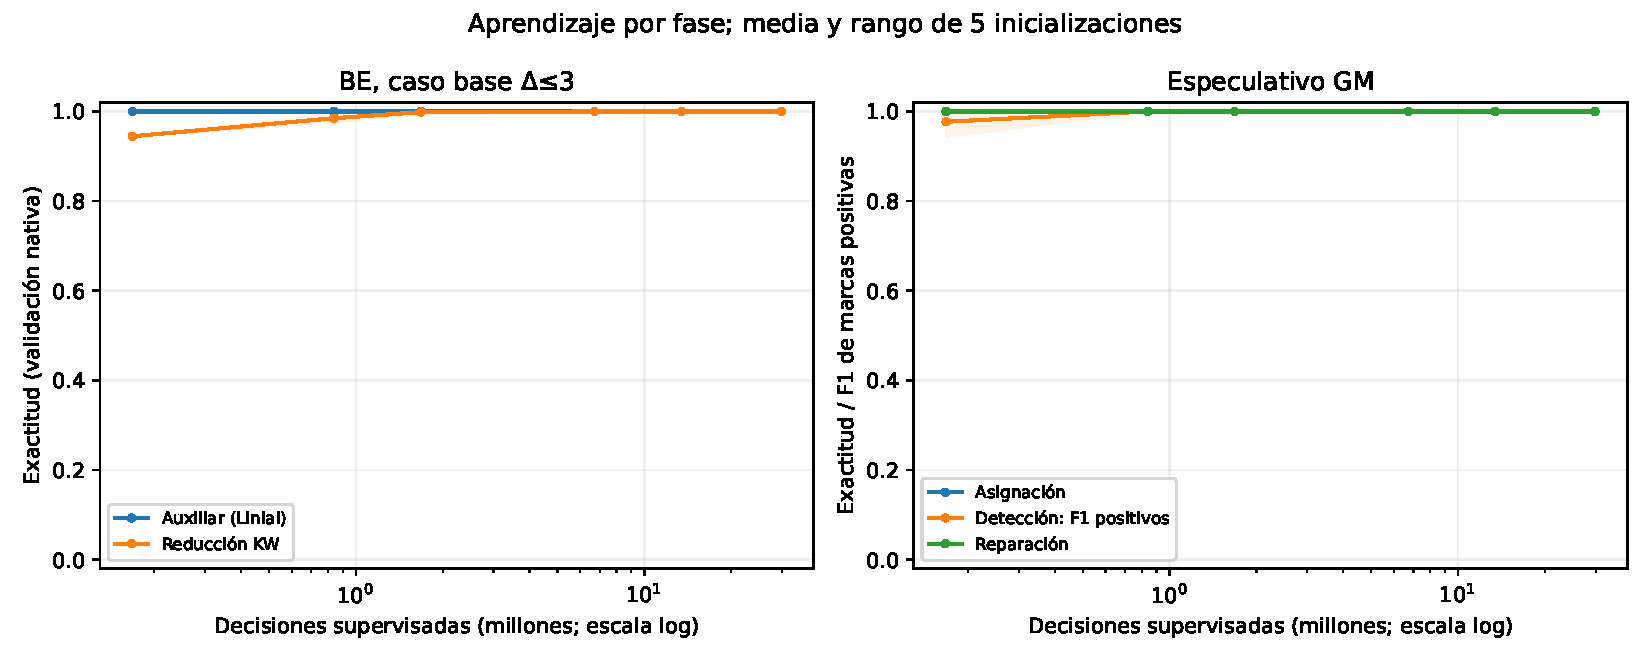
\includegraphics[width=\linewidth]{learning-by-phase.pdf}
\captionof{figure}{Aprendizaje por fase en la nueva cohorte. BE: elección del
punto auxiliar y reducción KW. GM: asignación, detección y reparación. En
detección se informa F1 de marcas positivas para evitar que los muchos negativos
dominen la exactitud. Media y rango de cinco inicializaciones.}
\end{center}

\subhead{Supervisión concordante con la propuesta evaluada}
En las fases de color se factoriza la decisión en participación, candidato y
confirmación. La pérdida es
\[
 L = L_P + L_C + \tfrac12 L_{\mathrm{COMMIT,propio}}
                 + \tfrac12 L_{\mathrm{COMMIT,CF}}.
\]
Durante las primeras 1.480 actualizaciones, la confirmación recibe propuestas
del maestro. Luego se recalculan las etiquetas para las propuestas de la red
y para propuestas contrafactuales: se enseña a confirmar o rechazar la
propuesta que efectivamente se está consultando.

Las inyecciones locales de conflicto usan probabilidades 0,17 contra colores
fijados y 0,04 entre propuestas simultáneas. ColorTrials y KW reciben también
consultas uniformes de candidato con probabilidad 0,5. BE-Linial aprende el
punto mediante entropía cruzada; GM-DETECT aprende una marca binaria mediante
BCE. Esas dos fases no tienen las tres decisiones originales de color.

\subhead{La estructura nativa está suministrada}
\begin{itemize}
\item \textbf{ColorTrials:} compara preferencias por color después de comunicar
disponibilidad aprendida. La selección se retrasa al segundo intercambio.
\item \textbf{BE:} el intérprete fija fases y representación polinomial. En KW
se dan comparaciones auxiliares por opción; la red aprende a agregarlas y decidir.
\item \textbf{GM:} el calendario de asignación y la reparación están programados.
La cola de reparación depende de las marcas predichas por la red.
\item \textbf{Greedy:} el orden secuencial está programado. El experimento mide
la decisión local de colorear, no aprender ese orden.
\end{itemize}

\begin{finding}
En inferencia, \textbf{se aplican las predicciones sin consultar al maestro
ni filtrar decisiones por validez}. La comprobación posterior de la coloración
detecta éxitos y fallos. La ayuda de representación de BE, que construye
$(x,p_v(x))$, sí forma parte explícita del modelo adaptado.
\end{finding}

{\small\color{muted}El contador heredado \texttt{unsafe\_own\_commits} registra
violaciones de la regla nativa de confirmación; no es una misma medida de
seguridad entre todos los maestros. El criterio principal verifica la
coloración completa.}

\clearpage
\pageheading{06 · MÉTODO Y TRAZABILIDAD}{Alcance de la evidencia y reproducción}

\begingroup\small
\begin{tabularx}{\linewidth}{@{}p{34mm}Y@{}}
\toprule
Elemento & Protocolo común y alcance\\
\midrule
Entrenamiento & 800 grafos REGULAR, $N=40$, $\Delta=3$, tres tapes.
Mismos pools inmutables que la comparación anterior y entre inicializaciones.\\
Presupuesto & 17.760 actualizaciones $\times$ 1.680 decisiones = 29.836.800
visitas muestreadas por modelo; muestreo con reemplazo, Adam, tasa 0,001.\\
Validación & 50 grafos para decisiones locales y cuatro para seguimiento
autónomo. Siempre se usa el último checkpoint prefijado.\\
Prueba & 396 casos por actor: $N\in\{40,160,640,2560,10240\}$, familias
REGULAR/IRREGULAR y controles PATH/CYCLE/K4. 197 identidades de grafo.\\
Ejecuciones & 13.860 aprendidas + 2.772 referencias exactas = 16.632.
Las cinco inicializaciones y las tapes reutilizan grafos.\\
Congelación & 35 checkpoints sellados el 22 de octubre, 17:13:39 UTC,
antes de ejecutar la nueva evaluación. Son casos de test ya publicados.\\
Semántica & Fases y relojes nativos suministrados. Los cuatro maestros
paralelos irreversibles paran al colisionar, con límite de 128 pasos;
el evaluador E1 original continúa tras choques y permite 256 rondas.\\
\bottomrule
\end{tabularx}
\endgroup

\subhead{Qué se comprobó}
La campaña registró \textbf{176 pruebas dirigidas aprobadas}. La auditoría
verificó los 35 modelos y reprodujo 105 rollouts nativos. Para las versiones
con núcleo original comparó 45 trazas y 2.308 decisiones con sus módulos
canónicos: diferencia máxima de logits 0 y mismas acciones. Las 2.772
coloraciones exactas de referencia coinciden con las anteriores.
La revisión científica independiente sigue pendiente.

Los 800 grafos de entrenamiento, 50 de validación local, cuatro de seguimiento
y 197 de test están separados por fingerprint etiquetado. Esto no excluye
isomorfismos. Los 10 fuentes originales y las 29 dependencias numéricas selladas
se conservaron. Una corrección de entrada KW previa al test quedó documentada;
los 35 modelos oficiales se entrenaron de nuevo desde cero, sin reutilizar pesos
del prefijo técnico. La compilación de este PDF no repite la campaña.

\subhead{Límites que cambian la interpretación}
\begin{itemize}
\item La comparación anterior/nueva cambia arquitectura, representación y
supervisión conjuntamente. Para separar causas hacen falta controles específicos.
\item Las repeticiones sobre un grafo están correlacionadas. En el extremo
hay tres grafos por familia; no se estima una garantía de fallo universal.
\item Los pasos de un greedy secuencial y los de un método paralelo miden
calendarios distintos. Los costes nativos no son una unidad LOCAL común ni
tiempo real comparable. BE solo cubre su caso base de grado a lo sumo 3;
ColorTrials usa la variante repetida de este proyecto.
\end{itemize}

\subhead{Fuentes del informe}
\begingroup\footnotesize
Directorio: \file{results/multiteacher-e1/2026-10-22/}. Tablas:
\file{architecture-comparison.csv}, \file{learning-milestones.csv}.
Curvas: \file{learning-curves.csv}, \file{learning-by-phase.csv}.
Auditorías: \file{audit.json}, \file{verification.json}; pesos sellados:
\file{frozen.json}. Definiciones: \file{E1.md},
\file{docs/MULTITEACHER_E1.md} y \file{docs/MULTITEACHER_E1_METRICAS.md}.
Datos completos: \file{data/multiteacher-e1-20261022/}.

Construir desde la raíz: \texttt{python3 }\file{experiments/build_multiteacher_e1_pdf.py}.
Verificar tablas y hashes sin escribir: añadir \file{--check}.
Fuentes del PDF: \file{INFORME.tex}, \file{report-tables.tex}; procedencia:
\file{pdf-manifest.json}. Base Git: \file{80f486e}; fuentes E1 de
\file{1d8857b}. Cambios de este seguimiento conservados localmente.
\endgroup

\end{document}
